\section{Motivation}
% \section{动机}
\label{sec:motivation}

AI agents combine model reasoning with external tools, memory, and long-running environments, such as Claude Code~\cite{anthropic2025claudecode}, Codex~\cite{openai2025codex}.
% AI 智能体将模型推理与外部工具、记忆和长时间运行的环境相结合，例如 Claude Code~\cite{anthropic2025claudecode}、Codex~\cite{openai2025codex}。
Agents operate through an \emph{AI agent harness}: software around the model that maintains the agent loop and session state, routes tool calls, mediates shell, file, and network access, and returns results or feedback to the model, improving agent performance while enforcing instructions and constraints~\cite{langchain-harness,fowler-harness}.
% 智能体通过一个 \emph{AI 智能体 harness} 运行：包裹模型的软件，它维护智能体循环和会话状态，路由工具调用，中介 shell、文件和网络访问，并将结果或反馈返回给模型，在执行指令和约束的同时提升智能体性能~\cite{langchain-harness,fowler-harness}。
A single tool invocation can run arbitrary scripts, browse untrusted content, call APIs, and touch many files~\cite{debenedetti2024agentdojo,zhan2024injecagent,chennabasappa2025llamafirewall}.
% 单个工具调用可以运行任意脚本、浏览不受信任的内容、调用 API，并触及许多文件~\cite{debenedetti2024agentdojo,zhan2024injecagent,chennabasappa2025llamafirewall}。
To improve task performance, safety, and compliance, projects often encode intent-level policy in natural-language files (\texttt{CLAUDE.md}, \texttt{AGENTS.md})~\cite{chatlatanagulchai2025manifests,santos2025claudeconfig,lulla2026agentsmd} or deterministic policy configurations.
% 为提高任务性能、安全性和合规性，项目通常在自然语言文件（\texttt{CLAUDE.md}、\texttt{AGENTS.md}）~\cite{chatlatanagulchai2025manifests,santos2025claudeconfig,lulla2026agentsmd}或确定性策略配置中编码意图级策略。
A \emph{policy} specifies what the agent should do (\emph{instructions}) or should not do (\emph{constraints}); we term its semantic meaning the agent's \emph{policy intent}.
% \emph{策略}指定智能体应该做什么（\emph{指令}）或不应该做什么（\emph{约束}）；我们将其语义含义称为智能体的 \emph{策略意图}。
This section presents an empirical study of 64~projects to characterize the gap between policy intent and enforcement and motivate the design of \sys{}.
% 本节展示对 64 个项目的实证研究，以表征策略意图与执行之间的鸿沟，并推动 \sys{} 的设计。

\subsection{Methodology}
% \subsection{方法论}
\label{sec:empirical}

We collected public GitHub repositories containing \texttt{CLAUDE.md} or \texttt{AGENTS.md}, prioritizing AI-agent projects created after 2025 and excluding non-code, inactive, fake-star, and stub repositories.
% 我们收集了包含 \texttt{CLAUDE.md} 或 \texttt{AGENTS.md} 的公开 GitHub 仓库，优先考虑 2025 年后创建的 AI 智能体项目，并排除非代码、不活跃、刷星和占位仓库。
The snapshot (2026-05-23 UTC) contains 64~repositories (median 20K GitHub stars, min 9.8K), 84 instruction files, and 2{,}116~extracted statements.
% 快照（2026-05-23 UTC）包含 64 个仓库（中位数 20K GitHub 星，最小 9.8K）、84 个指令文件和 2,116 条提取的语句。

Prior studies classify instruction-file contents at file or section-heading granularity~\cite{chatlatanagulchai2025manifests,chatlatanagulchai2025agentreadmes,santos2025claudeconfig,lulla2026agentsmd}; Zhang et al.~\cite{zhang2026guardrails} further show that negative constraints and positive policies have different effects.
% 先前的研究在文件或章节标题粒度上对指令文件内容进行分类~\cite{chatlatanagulchai2025manifests,chatlatanagulchai2025agentreadmes,santos2025claudeconfig,lulla2026agentsmd}；Zhang 等人~\cite{zhang2026guardrails}进一步表明否定约束和肯定指令具有不同的效果。
We analyze at the statement level to classify their enforcement requirements and quantify the context they need to become concrete rules.
% 我们在语句级别进行分析，以分类它们的执行要求，并量化它们需要成为具体规则的上下文。
A \emph{statement} is a coherent unit expressing one claim or constraint.
% 一条 \emph{语句}是表达一个主张或约束的连贯单元。
A two-pass LLM Agent-assisted pipeline extracted statements with source line ranges and four labels (content type, topic, enforcement level, context requirement).
% 一个两遍 LLM 智能体辅助流水线提取了带有源行范围和四个标签（内容类型、主题、执行级别、上下文要求）的语句。
A validation script verified full source coverage and verbatim span matching, and cross-checked by independent Claude and Codex agents.
% 一个验证脚本验证了完整的源覆盖和逐字跨度匹配，并由独立的 Claude 和 Codex 智能体交叉检查。
A stratified sample of 100~statements was independently reviewed by human annotators and verified the labels are correct.
% 100 条语句的分层样本由人工标注者独立审查并验证标签正确。
Table~\ref{tab:examples} collects representative statements that illustrate all four axes, and the labels \textbf{S1}--\textbf{S8} are referenced throughout.
% 表~\ref{tab:examples}收集了说明所有四个轴的代表性语句，标签 \textbf{S1}--\textbf{S8} 在全文中被引用。

\begin{table*}[t]
\caption{Representative corpus statements illustrating all four classification axes. Enforcement level and context requirement apply only to policies (---\,=\,not applicable).}
% \caption{说明所有四个分类轴的代表性语料库语句。执行级别和上下文要求仅适用于策略（---\,=\,不适用）。}
\label{tab:examples}
\centering
\small
\begin{tabular}{@{}clllll@{}}
\toprule
& \textbf{Statement} & \textbf{Type} & \textbf{Topic} & \textbf{Enforcement} & \textbf{Context} \\
% & \textbf{语句} & \textbf{类型} & \textbf{主题} & \textbf{执行} & \textbf{上下文} \\
\midrule
S1 & ``The backend uses Express with TypeScript.'' & Desc & Architecture & --- & --- \\
% S1 & "后端使用 Express 和 TypeScript。" & 描述 & 架构 & --- & --- \\
S2 & ``Always explain your reasoning before changes.'' & Dir & AI Integr. & Semantic & --- \\
% S2 & "总是在更改前解释你的推理。" & 策略 & AI 集成 & 语义 & --- \\
S3 & ``Prefer \texttt{const} over \texttt{let}.'' & Dir & Impl.\ Det. & Content & None \\
% S3 & "优先使用 \texttt{const} 而非 \texttt{let}。" & 策略 & 实现细节 & 内容 & 无 \\
S4 & ``Never push to main directly.'' & Dir & Dev.\ Proc. & Per-event & None \\
% S4 & "永不直接推送到 main。" & 策略 & 开发流程 & 单事件 & 无 \\
S5 & ``Never modify upstream source code.'' & Dir & Dev.\ Proc. & Per-event & Project \\
% S5 & "永不修改上游源代码。" & 策略 & 开发流程 & 单事件 & 项目 \\
S6 & ``Run the full test suite before committing.'' & Dir & Testing & Cross-event & Project \\
% S6 & "提交前运行完整测试套件。" & 策略 & 测试 & 跨事件 & 项目 \\
S7 & ``Data read from \texttt{.env} must not reach the network.'' & Dir & Security & Cross-event & Project \\
% S7 & "从 \texttt{.env} 读取的数据不得到达网络。" & 策略 & 安全 & 跨事件 & 项目 \\
S8 & ``Do not update dependencies without approval.'' & Dir & Maint. & Per-event & Task \\
% S8 & "未经批准不要更新依赖。" & 策略 & 维护 & 单事件 & 任务 \\
\bottomrule
\end{tabular}
\Description{Table of eight representative statements from the corpus, each classified by type, topic, enforcement level, and context requirement.}
% \Description{语料库中八条代表性语句的表格，每条按类型、主题、执行级别和上下文要求分类。}
\end{table*}

\subsection{Are Instruction Files Behavioral Policies?}
% \subsection{指令文件是行为策略吗？}

A statement is a \emph{policy} if it asks the agent to perform, avoid, or condition an action, and is otherwise descriptive context.
% 如果一条语句要求智能体执行、避免或条件化一个行为，它就是一条 \emph{策略}，否则是描述性上下文。
Of the 2{,}116~statements, 1{,}361 (64.3\%) are policies and 755 (35.7\%) are descriptions (Figure~\ref{fig:empirical-rq1}).
% 在 2,116 条语句中，1,361 条（64.3\%）是策略，755 条（35.7\%）是描述（图~\ref{fig:empirical-rq1}）。

\noindent\textbf{Instruction files are mainly policies, with the median repository at 71\%.}
% \noindent\textbf{指令文件主要是策略，中位数仓库达到 71\%。}
75\% of repositories have a policy fraction above 50\%.
% 75\% 的仓库有超过 50\% 的策略比例。
At the extremes, one repository is entirely descriptive (0\% policies) while another is 97\% policies.
% 在极端情况下，一个仓库完全是描述性的（0\% 策略），而另一个是 97\% 策略。
This majority is invisible at line level because policies average 3.6 lines per statement while descriptions average 6.8 lines, so the same files appear balanced (49\% policies) when measured by lines.
% 这个多数在行级别是不可见的，因为策略平均每条语句 3.6 行而描述平均 6.8 行，所以同样的文件在按行测量时显得平衡（49\% 策略）。

\begin{figure}[t]
\centering
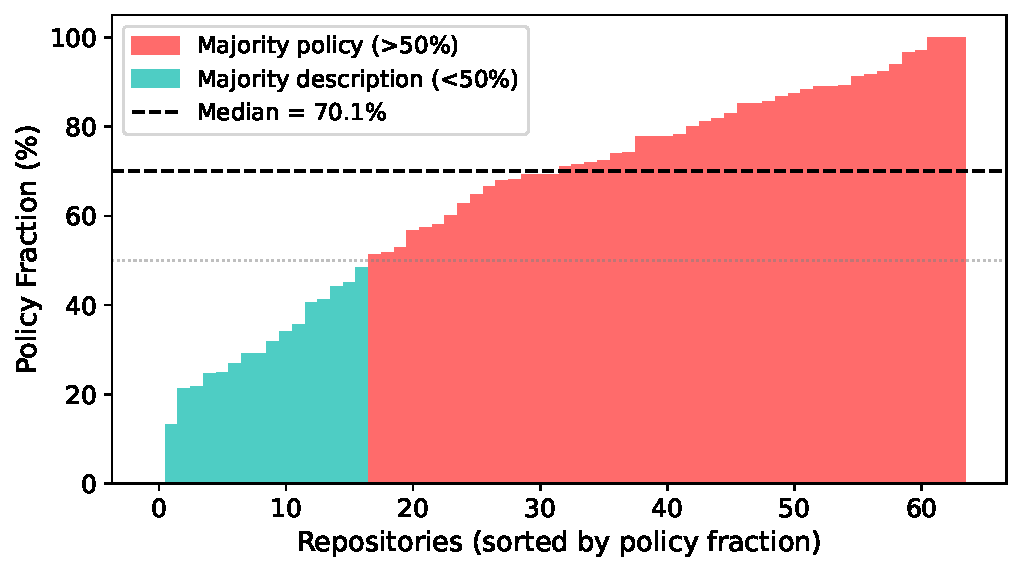
\includegraphics[width=\columnwidth]{figures/empirical_rq1_policy_fraction.pdf}
\caption{Policy fraction per repository by statement count. Most repositories contain a majority of policy statements.}
% \caption{按语句数量计算的每个仓库的策略比例。大多数仓库包含多数策略语句。}
\Description{Sorted bar chart of policy fraction per repository.}
% \Description{每个仓库策略比例的排序条形图。}
\label{fig:empirical-rq1}
\end{figure}

\subsection{Which Topics Contain Policies?}
% \subsection{哪些主题包含策略？}

Each statement is assigned to one of 12~topic categories adapted from prior instruction-file studies~\cite{chatlatanagulchai2025agentreadmes}, applied at statement granularity rather than file granularity (Figure~\ref{fig:empirical-rq2}).
% 每条语句被分配到 12 个主题类别之一，这些类别改编自先前的指令文件研究~\cite{chatlatanagulchai2025agentreadmes}，应用于语句粒度而非文件粒度（图~\ref{fig:empirical-rq2}）。

\noindent\textbf{Policy density ranges from 0\% (System Overview) to 87\% (Development Process).}
% \noindent\textbf{策略密度从 0\%（系统概述）到 87\%（开发流程）不等。}
Development Process and Implementation Details are policy-heavy (86.7\% and 85.2\%, respectively).
% 开发流程和实现细节是策略密集的（分别为 86.7\% 和 85.2\%）。
Architecture is mostly descriptive because directory layouts and design summaries make it one of the largest topics by line count, yet only 23.0\% of its statements are policies.
% 架构主要是描述性的，因为目录布局和设计摘要使其按行数成为最大的主题之一，然而只有 23.0\% 的语句是策略。

\begin{figure}[t]
\centering
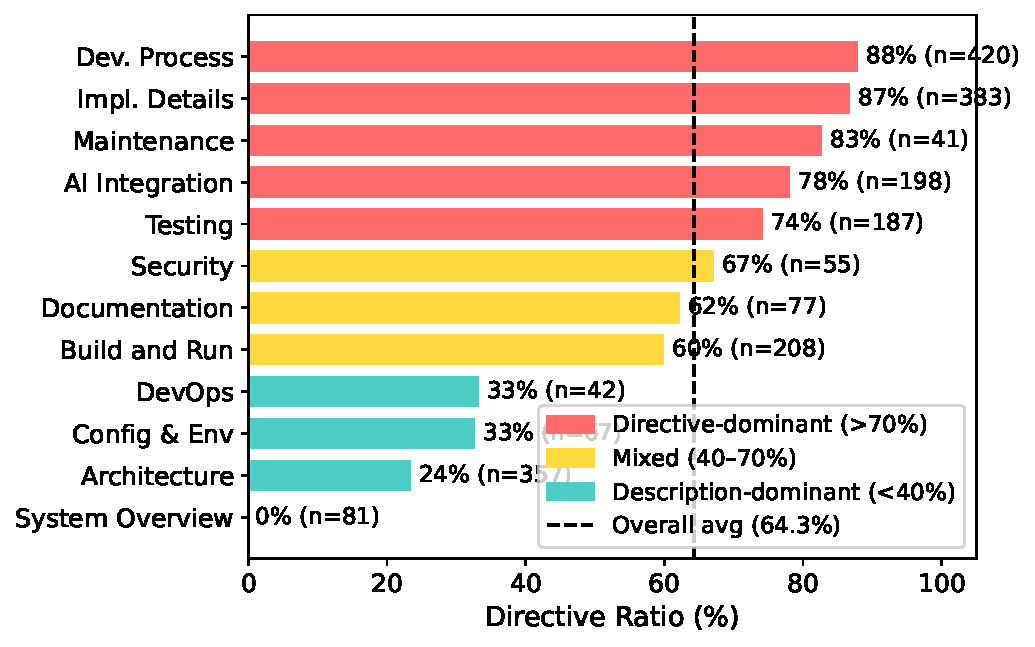
\includegraphics[width=\columnwidth]{figures/empirical_rq2_policy_ratio.pdf}
\caption{Policy ratio by topic.}
% \caption{按主题的策略比例。}
\Description{Bar chart showing policy ratio for each topic.}
% \Description{显示每个主题策略比例的条形图。}
\label{fig:empirical-rq2}
\end{figure}

\subsection{Which Policies Require OS-Level Enforcement?}
% \subsection{哪些策略需要操作系统级执行？}

We use \emph{runtime policy enforcement system} for the part of an AI agent harness that enforces safety, security, and compliance policies while the agent executes.
% 我们使用 \emph{运行时策略执行系统}指代 AI 智能体 harness 中在智能体执行时执行安全、安全性和合规策略的部分。
Existing enforcement operates at three levels.
% 现有执行在三个级别运行。
Prompt instructions rely on the model's own compliance capabilities~\cite{liu2024lost,jiang2024followbench,qi2025agentif} and are vulnerable to prompt injection~\cite{greshake2023indirectprompt,zhan2024injecagent,debenedetti2024agentdojo}.
% 提示词指令依赖于模型自身的遵循能力~\cite{liu2024lost,jiang2024followbench,qi2025agentif}，并且容易受到提示词注入攻击~\cite{greshake2023indirectprompt,zhan2024injecagent,debenedetti2024agentdojo}。
Separate agents or LLM guards can check prompts, responses, or action trajectories at runtime~\cite{rebedea2023nemo,xiang2025guardagent,chennabasappa2025llamafirewall} but are inherently probabilistic.
% 独立的智能体或 LLM 守卫可以在运行时检查提示词、响应或行为轨迹~\cite{rebedea2023nemo,xiang2025guardagent,chennabasappa2025llamafirewall}，但本质上是概率性的。
Tool-call guardrails and application-level IFC systems~\cite{wang2025agentspec,shi2025progent,invariant-guardrails,costa2025fides,debenedetti2025camel} intercept at the harness boundary deterministically, but these three levels observe only harness-mediated requests, not the system-level effects once a tool starts executing, so an indirect subprocess, a shell-out, or a compiled binary can bypass the tool boundary.
% 工具调用护栏和应用级 IFC 系统~\cite{wang2025agentspec,shi2025progent,invariant-guardrails,costa2025fides,debenedetti2025camel}在 harness 边界确定性地拦截，但这三个级别仅观察 harness 中介的请求，而不是工具开始执行后的系统级效果，因此间接子进程、shell 调用或编译的二进制文件可以绕过工具边界。
OS-level mechanisms (seccomp~\cite{seccomp-bpf}, AppArmor~\cite{apparmor}, Capsicum~\cite{watson2010capsicum}, Landlock~\cite{landlock}, BPF-LSM~\cite{linuxbpflsm}, Tetragon~\cite{ciliumtetragon}, KubeArmor~\cite{kubearmor}, and BPFContain~\cite{findlay2021bpfcontain}) restrict process, file, and network access below the tool layer and are increasingly adopted as agent sandboxes, but they expect statically pre-written policies and return opaque errors with no connection to policy intent.
% 操作系统级机制（seccomp~\cite{seccomp-bpf}、AppArmor~\cite{apparmor}、Capsicum~\cite{watson2010capsicum}、Landlock~\cite{landlock}、BPF-LSM~\cite{linuxbpflsm}、Tetragon~\cite{ciliumtetragon}、KubeArmor~\cite{kubearmor} 和 BPFContain~\cite{findlay2021bpfcontain}）在工具层之下限制进程、文件和网络访问，并越来越多地被采用为智能体沙箱，但它们期望静态预写的策略，并返回与策略意图没有连接的不透明错误。

Each policy is classified into the first matching tier of an enforcement waterfall (Figure~\ref{fig:waterfall-enforcement}): \emph{semantic-only} (reasoning, communication, or output style), \emph{content} (predicates over file contents), \emph{per-event} (a single command, file access, or network connection), and \emph{cross-event} (history, ordering, lineage, or information flow).
% 每条策略被分类到执行瀑布的第一个匹配层级（图~\ref{fig:waterfall-enforcement}）：\emph{仅语义}（推理、沟通或输出风格）、\emph{内容}（文件内容上的谓词）、\emph{单事件}（单个命令、文件访问或网络连接）和 \emph{跨事件}（历史、顺序、血统或信息流）。
We call the union of content, per-event, and cross-event policies \emph{system-observable}, and the per-event and cross-event subset that \sys{} can enforce at OS hooks is \emph{OS-enforceable}.
% 我们将内容、单事件和跨事件策略的并集称为 \emph{系统可观察}，\sys{} 可以在操作系统钩子上执行的单事件和跨事件子集是 \emph{操作系统可执行}。

\noindent\textbf{83\% of policies constrain system actions.}
% \noindent\textbf{83\% 的策略约束系统行为。}
Of 1{,}361~policies, 234 (17.2\%) are semantic-only, 520 (38.2\%) require content inspection, 392 (28.8\%) match a single OS event, and 215 (15.8\%) require cross-event state (Table~\ref{tab:examples}, S2--S7 illustrate all four levels).
% 在 1,361 条策略中，234 条（17.2\%）是仅语义的，520 条（38.2\%）需要内容检查，392 条（28.8\%）匹配单个操作系统事件，215 条（15.8\%）需要跨事件状态（表~\ref{tab:examples}，S2--S7 说明所有四个级别）。
Content inspection alone covers 55.4\% of policies, adding per-event matching reaches 84.2\%, and the remaining 15.8\% require cross-event IFC.
% 仅内容检查覆盖 55.4\% 的策略，加上单事件匹配达到 84.2\%，剩余的 15.8\% 需要跨事件 IFC。

\noindent\textbf{Cross-event policies concentrate in Development Process, which accounts for 39.5\% of all cross-event policies (Figure~\ref{fig:enforcement-by-topic}).}
% \noindent\textbf{跨事件策略集中在开发流程，占所有跨事件策略的 39.5\%（图~\ref{fig:enforcement-by-topic}）。}
Four recurring patterns emerge, including temporal ordering (``run tests before committing''), cross-file consistency (``update docs when behavior changes''), multi-step workflows (release checklists with verification steps), and conditional triggers (``if you change specs, also update SDK'').
% 出现四种反复模式，包括时间顺序（"提交前运行测试"）、跨文件一致性（"行为变化时更新文档"）、多步骤工作流（带有验证步骤的发布清单）和条件触发器（"如果你更改规范，也要更新 SDK"）。
All four require state that spans multiple operations, tracking what ran, in what order, and what has changed since.
% 所有四种都需要跨越多个操作的状态，追踪运行了什么、以什么顺序、以及从那时起发生了什么变化。
Most of the operations involve files, processes, and network connections.
% 大多数操作涉及文件、进程和网络连接。

\noindent\textbf{At the repository level, 81\% of repositories contain at least one cross-event policy, and 43\% require all four enforcement layers.}
% \noindent\textbf{在仓库级别，81\% 的仓库包含至少一条跨事件策略，43\% 需要所有四个执行层级。}

\begin{figure}[t]
\centering
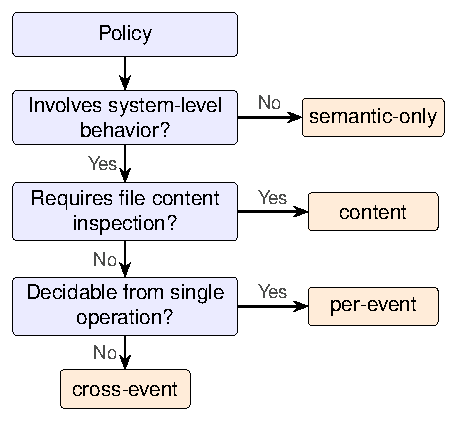
\includegraphics[width=0.85\columnwidth]{figures/empirical-waterfall-enforcement.pdf}
\caption{Enforcement-level waterfall. Each policy exits at the first matching tier.}
% \caption{执行级别瀑布。每条策略在第一个匹配层级退出。}
\Description{Flowchart showing the enforcement-level waterfall decision procedure with four outcomes: semantic-only, content, per-event, cross-event.}
% \Description{显示执行级别瀑布决策过程的流程图，有四个结果：仅语义、内容、单事件、跨事件。}
\label{fig:waterfall-enforcement}
\end{figure}

\begin{figure}[t]
\centering
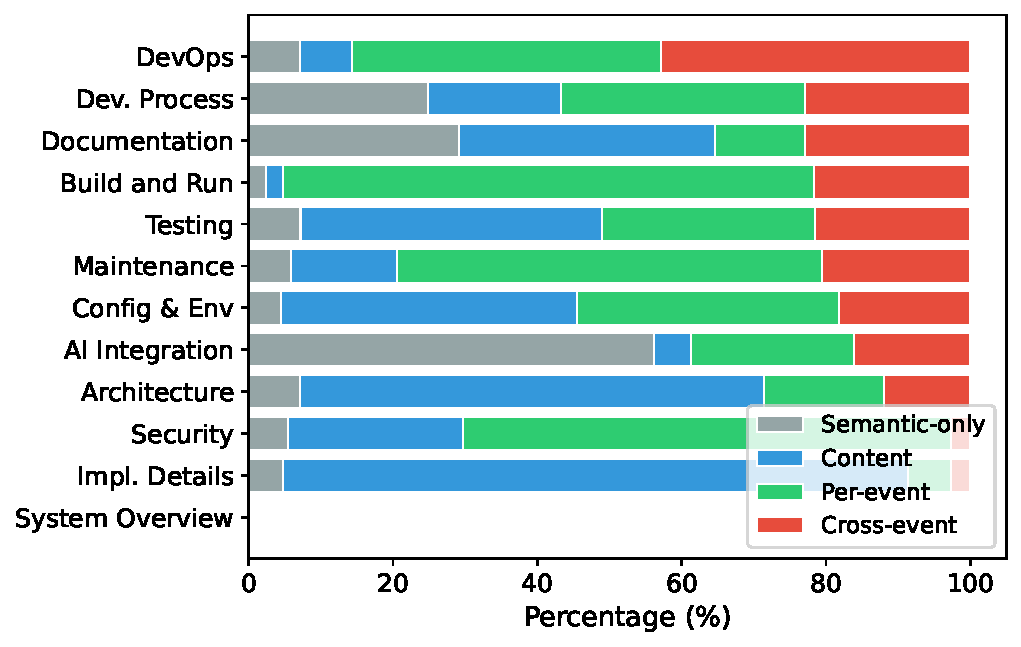
\includegraphics[width=\columnwidth]{figures/empirical_rq3_enforcement_by_topic.pdf}
\caption{Enforcement profile by topic (normalized). Topics exhibit distinct archetypes, and cross-event policies concentrate in Development Process.}
% \caption{按主题的执行概况（归一化）。主题呈现出不同的原型，跨事件策略集中在开发流程。}
\Description{Stacked horizontal bar chart showing the normalized enforcement-level breakdown for each topic category.}
% \Description{显示每个主题类别的归一化执行级别分布的堆叠水平条形图。}
\label{fig:enforcement-by-topic}
\end{figure}

\subsection{What Context Is Needed to Instantiate Rules?}
% \subsection{实例化规则需要什么上下文？}

Each system-observable policy is classified by what additional context an enforcement mechanism needs beyond the policy text itself (Figure~\ref{fig:waterfall-context}): \emph{self-contained} if all commands, paths, and patterns are explicit; \emph{project context} if it references an unresolved repository-specific concept (``the full test suite,'' ``the migration tool''); or \emph{task context} if it depends on the current user request or a per-session grant (``unless explicitly requested,'' ``without approval'').
% 每条系统可观察的策略按执行机制除了策略文本本身还需要什么额外上下文来分类（图~\ref{fig:waterfall-context}）：如果所有命令、路径和模式都是显式的，则为 \emph{自包含}；如果它引用一个未解析的仓库特定概念（"完整测试套件"、"迁移工具"），则为 \emph{项目上下文}；如果它依赖于当前用户请求或每会话授权（"除非明确请求"、"未经批准"），则为 \emph{任务上下文}。

\noindent\textbf{74\% of system-observable policies require project or task context to instantiate as concrete rules.}
% \noindent\textbf{74\% 的系统可观察策略需要项目或任务上下文才能实例化为具体规则。}
Of the 1{,}127~system-observable policies, only 26.4\% are self-contained.
% 在 1,127 条系统可观察的策略中，只有 26.4\% 是自包含的。
Another 64.2\% require project context because the policy mentions ``the test suite,'' ``the linter,'' or ``upstream source,'' whose concrete command or path needs to be resolved from the repository.
% 另外 64.2\% 需要项目上下文，因为策略提到"测试套件"、"代码检查器"或"上游源码"，其具体命令或路径需要从仓库中解析。
The remaining 9.4\% require task context (Figure~\ref{fig:empirical-rq4}; Table~\ref{tab:examples}: S4 is self-contained; S5--S7 require project context; S8 requires task context).
% 剩余 9.4\% 需要任务上下文（图~\ref{fig:empirical-rq4}；表~\ref{tab:examples}：S4 是自包含的；S5--S7 需要项目上下文；S8 需要任务上下文）。

\noindent\textbf{Cross-event policies are 95\% context-dependent, compared to 58\% for content policies.}
% \noindent\textbf{跨事件策略 95\% 依赖上下文，相比之下内容策略为 58\%。}
Of cross-event policies, 76.7\% require project context and 18.6\% task context (95.3\% total), while content policies are only 57.5\% context-dependent.
% 在跨事件策略中，76.7\% 需要项目上下文，18.6\% 需要任务上下文（共 95.3\%），而内容策略只有 57.5\% 依赖上下文。
This compounds the enforcement challenge because policies that require cross-event IFC rarely specify the concrete commands and paths needed to write the rule.
% 这加剧了执行挑战，因为需要跨事件 IFC 的策略很少指定编写规则所需的具体命令和路径。
Generic static rules can cover only the self-contained fraction, and the majority require the agent itself to read the repository, interpret the current task, and produce a concrete policy before enforcement begins.
% 通用静态规则只能覆盖自包含的部分，大多数需要智能体自己读取仓库、解释当前任务，并在执行开始前生成具体策略。

\begin{figure}[t]
\centering
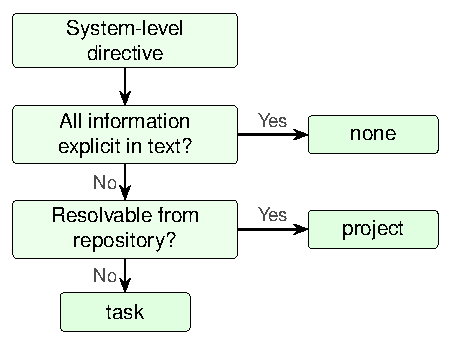
\includegraphics[width=0.78\columnwidth]{figures/empirical-waterfall-context.pdf}
\caption{Context-requirement waterfall. Each system-level policy exits at the first matching tier.}
% \caption{上下文要求瀑布。每条系统级策略在第一个匹配层级退出。}
\Description{Flowchart showing the context-requirement waterfall with three outcomes: none, project, task.}
% \Description{显示上下文要求瀑布的流程图，有三个结果：无、项目、任务。}
\label{fig:waterfall-context}
\end{figure}

\begin{figure}[t]
\centering
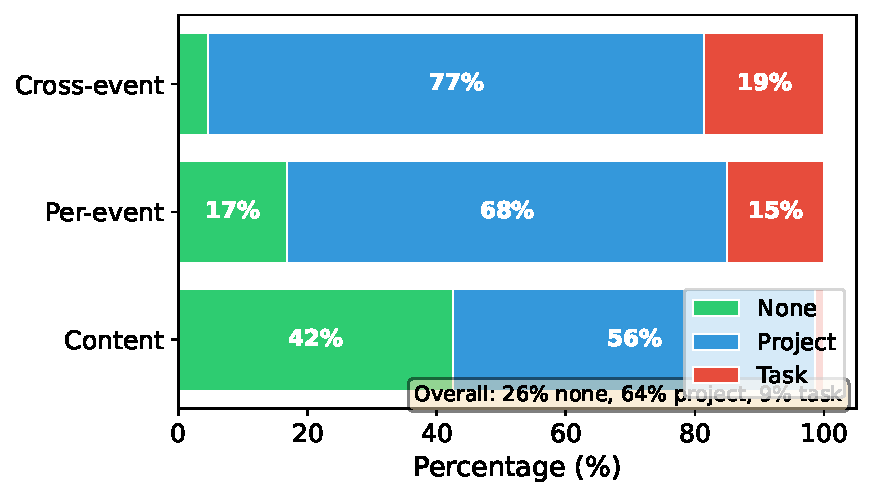
\includegraphics[width=\columnwidth]{figures/empirical_rq4_context_by_enforcement.pdf}
\caption{Context requirement by enforcement level. Cross-event policies are 95\% context-dependent, while content policies are 42\% self-contained.}
% \caption{按执行级别的上下文要求。跨事件策略 95\% 依赖上下文，而内容策略 42\% 是自包含的。}
\Description{Stacked horizontal bar chart showing context requirement (none, project, task) for each enforcement level.}
% \Description{显示每个执行级别的上下文要求（无、项目、任务）的堆叠水平条形图。}
\label{fig:empirical-rq4}
\end{figure}

\subsection{Design Requirements}
% \subsection{设计要求}

These findings establish two requirements for a policy engine in AI agent harnesses.
% 这些发现为 AI 智能体 harness 中的策略引擎确立了两项要求。

\emph{R1: agent-writable, OS-enforceable policy specification.}
% \emph{R1：智能体可编写的、操作系统可执行的策略规范。}
Most rules need project or task context that resides with the agent (E-RQ4), so the agent itself must be able to turn policies into concrete rules, and it needs semantic feedback to understand violations and recover.
% 大多数规则需要存在于智能体处的项目或任务上下文（E-RQ4），因此智能体自身必须能够将策略转化为具体规则，并且它需要语义反馈来理解违规并恢复。
Yet many policies constrain system actions that span multiple operations and are invisible to tool-call guardrails (E-RQ3), so the rules must be concrete enough for deterministic OS-level cross-event enforcement.
% 然而许多策略约束跨越多个操作的系统行为，这对工具调用护栏是不可见的（E-RQ3），因此规则必须足够具体以进行确定性操作系统级跨事件执行。

\emph{R2: safe, isolated, and efficient enforcement.}
% \emph{R2：安全的、隔离的和高效的执行。}
Enforcement must hold under probabilistic errors or prompt injection, agent-authored policy must not weaken safety constraints set by higher authority or affect other agents' policies, and enforcement must not slow the agent's normal workload.
% 执行必须在概率错误或提示词注入下保持，智能体编写的策略不能削弱由更高权限设置的安全约束或影响其他智能体的策略，并且执行不能减慢智能体的正常工作负载。
